\section{Casi d'uso}\label{sec:casi-d'uso}
\subsection{UC-1 Selezione file}\label{subsec:uc-1-selezione-file}
\begin{itemize}
    \item \textbf{attori:} utente generico;
    \item \textbf{scopo:} permettere all'utente di selezionare il file APK da analizzare;
    \item \textbf{descrizione:} serve per permettere all'utente di selezionare il file APK da analizzare;
    \item \textbf{pre-condizioni:} l'utente ha avviato il tool;
    \item \textbf{post-condizioni:} l'utente ha selezionato un file di con estensione \gls{APK} valido;
    \item \textbf{flusso degli eventi principali:}
    \begin{itemize}
        \item l'utente seleziona il file;
        \item l'utente conferma la selezione del file.
    \end{itemize}
\end{itemize}
\subsection{UC-2 Avvio decompilazione}\label{subsec:uc-2-avvio-decompilazione}
\begin{itemize}
    \item \textbf{attori:} utente generico;
    \item \textbf{scopo:} serve per avviare la decompilazione;
    \item \textbf{descrizione:} l'utente deve avviare la decompilazione del file APK;
    \item \textbf{pre-condizioni:} l'utente ha selezionato con successo un file APK;
    \item \textbf{post-condizioni:} la decompilazione è avvenuto con successo;
    \item \textbf{flusso degli eventi principali:}
    \begin{itemize}
        \item l'utente avvia la decompilazione;
        \item l'utente visualizza il messaggio della decompilazione avvenuto con successo;
    \end{itemize}
    \item \textbf{Estensione:}
    \begin{itemize}
        \item UC-3 Visualizzazione errore di decompilazione;
    \end{itemize}
\end{itemize}

\subsection{UC-3 Visualizzazione errore di decompilazione}\label{subsec:uc-3-visualizzazione-errore-di-decompilazione}
\begin{itemize}
    \item \textbf{attori:} utente generico;
    \item \textbf{scopo:} mostrare il messaggio d'errore della decompilazione;
    \item \textbf{descrizione:} la decompilazione del file APK potrebbe generare degli errori;
    \item \textbf{pre-condizioni:} l'utente ha avviato la decompilazione dell'APK;
    \item \textbf{post-condizioni:} l'utente ha visualizzato il messaggio d'errore;
    \item \textbf{flusso degli eventi principali:}
    \begin{itemize}
        \item l'utente visualizza il messaggio di errore;
    \end{itemize}
\end{itemize}
\subsection{UC-4 Installazione APK decompilato}\label{subsec:uc-4-installazione-apk-decompilato}
\begin{itemize}
    \item \textbf{attori:} utente generico;
    \item \textbf{scopo:} installazione dell'APK decompilato su un AVD;
    \item \textbf{descrizione:} permette all'utente d'installare l'apk, decompilato, manomesso e ricompilato, su un AVD;
    \item \textbf{pre-condizioni:} la decompilazione dell'APK è stato eseguito con successo;
    \item \textbf{post-condizioni:} l'APK è stato installato sull'AVD con successo;
    \item \textbf{flusso degli eventi principali:}
    \begin{itemize}
        \item l'utente seleziona un'AVD presente sul proprio computer;
        \item l'utente avvia l'installazione dell'APK ricompilato;
        \item l'utente visualizza un messaggio d'installazione avvenuto con successo;
    \end{itemize}
\end{itemize}
\subsubsection{UC-4.1 Selezione AVD}\label{subsubsec:uc-4.1-selezione-avd}
\begin{itemize}
    \item \textbf{attori:} utente generico;
    \item \textbf{scopo:} permettere all'utente di selezionare i AVD presenti nel proprio computer;
    \item \textbf{descrizione:} serve per permettere all'utente di selezionare un'AVD presente nel proprio computer;
    \item \textbf{pre-condizioni:} l'utente ha avviato il software;
    \item \textbf{post-condizioni:} l'utente ha selezionato l'AVD da avviare;
    \item \textbf{flusso degli eventi principali:}
    \begin{itemize}
        \item l'utente visualizza un elenco delle AVD presenti nel proprio computer;
        \item l'utente seleziona un'AVD;
        \item l'utente conferma la selezione;
        \item l'AVD selezionato si è avviato con successo
    \end{itemize}
    \item \textbf{Estensione}
    \begin{itemize}
        \item UC-5 Visualizzazione messaggio nessun AVD rilevato;
    \end{itemize}
\end{itemize}
\begin{figure}
    \centering
    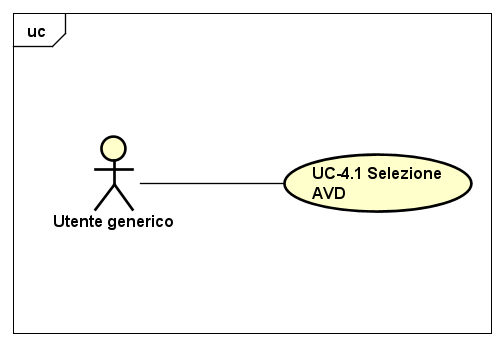
\includegraphics[width=10cm, height=8cm]{./usecase/uc_4_1.png}
    \caption{UC-4.1 Selezione AVD}
\end{figure}

\subsection{UC-5 Visualizzazione messaggio nessun AVD rilevato} \label{subsec:uc-5-visualizzazione-messaggio-nessun-avd-rilevato}
\begin{itemize}
    \item \textbf{attori:} utente generico;
    \item \textbf{scopo:} mostrare all'utente che non sono stati rilevati alcun AVD;
    \item \textbf{descrizione:} quando non sono presenti nessun AVD o il tool non è riuscito a rilevarne, viene mostrato un messaggio all'utente;
    \item \textbf{pre-condizioni:} l'utente ha aperto il tool;
    \item \textbf{post-condizioni:} l'utente ha visualizzato il messaggio;
    \item \textbf{flusso degli eventi principali:}
    \begin{itemize}
        \item l'utente visualizza il messaggio;
    \end{itemize}
\end{itemize}
\subsection{UC-6 Errore durante avvio dell'AVD}\label{subsec:uc-6-errore-durante-avvio-dell'avd}
\begin{itemize}
    \item \textbf{attori:} utente generico;
    \item \textbf{scopo:} mostrare all'utente gli eventuali errori durante l'avvio dell'AVD;
    \item \textbf{descrizione:} serve a mostrare all'utente gli eventuali errori durante l'avvio dell'AVD;
    \item \textbf{pre-condizioni:} l'utente ha selezionato un'AVD e ha confermato l'avvio;
    \item \textbf{post-condizioni:} l'utente ha visualizzato il messaggio d'errore;
    \item \textbf{flusso degli eventi principali:}
    \begin{itemize}
        \item l'utente visualizza il messaggio d'errore;
    \end{itemize}
\end{itemize}
\subsection{UC-7 Dump dello storage interno}\label{subsec:uc-6-dump-dello-storage-interno}
\begin{itemize}
    \item \textbf{attori:} utente generico;
    \item \textbf{scopo:} permettere all'utente di fare il dump dello storage interno;
    \item \textbf{descrizione:} nel caso l'utente volesse una copia dei dati interni dell'applicativo, ha bisogno di fare il dump;
    \item \textbf{pre-condizioni:} l'installazione dell'APK manomesso è andato a buon fine;
    \item \textbf{post-condizioni:} è stato fatto una copia dello storage interno;
    \item \textbf{flusso degli eventi principali:}
    \begin{itemize}
        \item l'utente seleziona la voce "copia i dati interni";
        \item l'utente seleziona il path dove collocare i dati;
    \end{itemize}
\end{itemize}
\subsection{UC-8 Decodifica del codice}\label{subsec:uc-8-decodifica-del-codice}
\begin{itemize}
    \item \textbf{attori:} utente generico;
    \item \textbf{scopo:} permettere all'utente di effettuare la decodifica dei file \textbf{.dex} in codice \textbf{.java};
    \item \textbf{descrizione:} durante la decompilazione dell'APK vengono creati dei file .dex che contengono il codice sorgente dell'APK, e questo caso d'uso serve per permettere all'utente di ottenere il codice sorgente;
    \item \textbf{pre-condizioni:} la decompilazione è avvenuto con successo;
    \item \textbf{post-condizioni:} l'utente ha ottenuto una copia del codice sorgente in java;
    \item \textbf{flusso degli eventi principali:}
    \begin{itemize}
        \item l'utente ha selezionato la funzionalità decodifica dei dex;
        \item l'utente seleziona il percorso dove posizionare il codice sorgente ottenuto;
        \item l'utente ha salvato il codice sorgente ottenuto.
    \end{itemize}
\end{itemize}
\subsubsection{UC-8.1 Avvio decodifica}
\begin{itemize}
    \item \textbf{attori:} utente generico;
    \item \textbf{scopo:} serve all'utente per avviare la decodifica dei file .dex;
    \item \textbf{descrizione:} serve all'utente per avviare la decodifica dei file .dex;
    \item \textbf{pre-condizioni:} la decompilazione dell'APK è avvenuto correttamente;
    \item \textbf{post-condizioni:} la decodifica è avvenuto con successo;
    \item \textbf{flusso degli eventi principali:}
    \begin{itemize}
        \item l'utente seleziona la funzionalità di decodifica dei file .dex;
    \end{itemize}
\end{itemize}
\subsubsection{UC-8.2 Salvataggio del codice decodificato}
\begin{itemize}
    \item \textbf{attori:} utente generico;
    \item \textbf{scopo:} serve all'utente per salvare i codici sorgenti decodificati;
    \item \textbf{descrizione:} serve all'utente per salvare i codici sorgenti decodificati;
    \item \textbf{pre-condizioni:} la decompilazione è avvenuto con successo;
    \item \textbf{post-condizioni:} i file con i codici sorgenti sono stati salvati correttamente;
    \item \textbf{flusso degli eventi principali:}
    \begin{itemize}
        \item l'utente seleziona la voce "salva file decodificati";
        \item l'utente seleziona la posizione dove vuole salvare i file;
        \item i file vengono salvati correttamente.
    \end{itemize}
\end{itemize}

\begin{figure}[H]
    \centering
    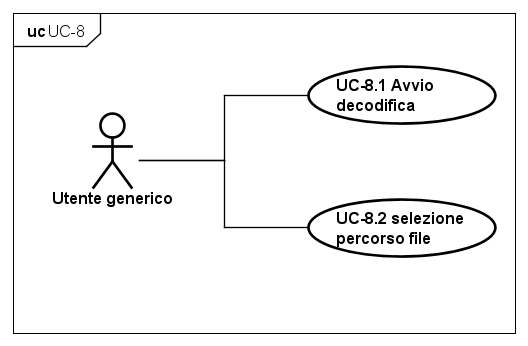
\includegraphics[width=10cm, height=8cm]{./immagini/usecase/uc_8.png}
    \caption{UC-8 Decodifica codici .dex}
\end{figure}



\subsection{UC-9 Visualizzazione errore decodifica}\label{subsec:uc-9-visualizzazione-errore-decodifica}
\begin{itemize}
    \item \textbf{attori:} utente generico;
    \item \textbf{scopo:} mostrare all'utente il messaggio di errore di decodifica del .dex;
    \item \textbf{descrizione:} durante la decodifica dei .dex possono sorgere molteplici errori;
    \item \textbf{pre-condizioni:} l'utente ha selezionato la funzionalità di decodifica del codice .dex;
    \item \textbf{post-condizioni:} l'utente ha visualizzato il messaggio di errore durante la decodifica;
    \item \textbf{flusso degli eventi principali:}
    \begin{itemize}
        \item l'utente ha visualizzato il messaggio d'errore;
    \end{itemize}
\end{itemize}

\begin{figure}[H]
    \centering
    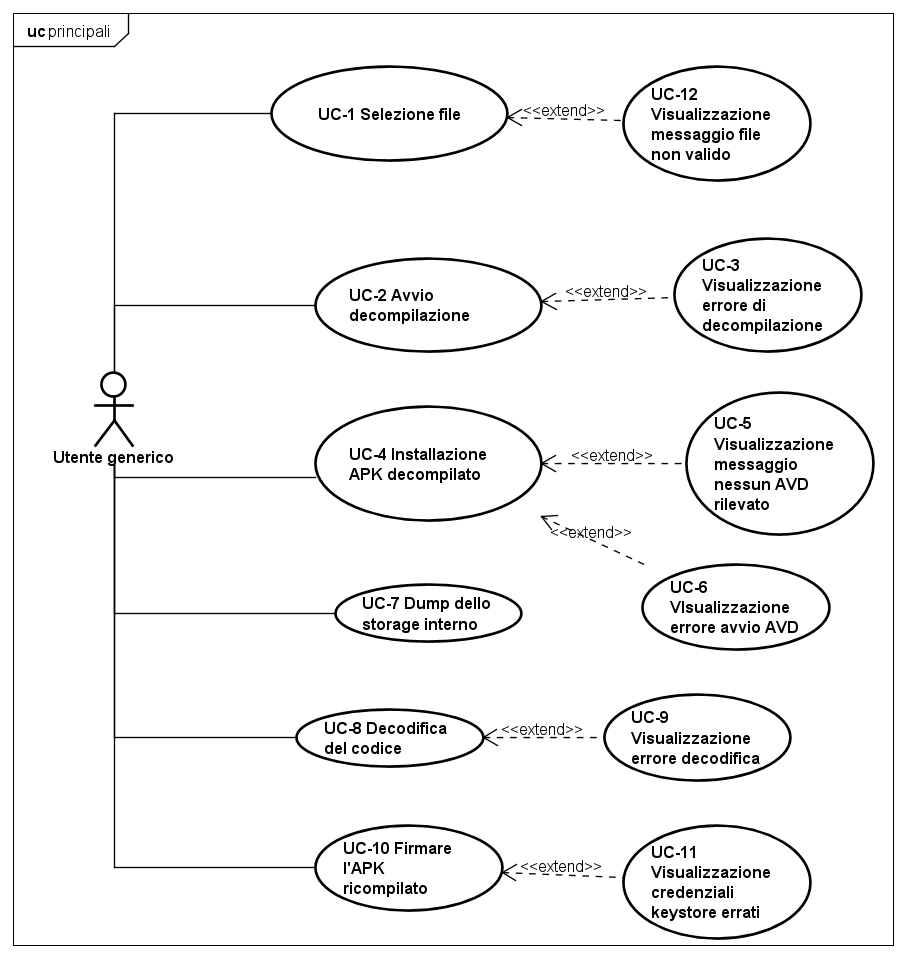
\includegraphics[width=10cm, height=8cm]{./immagini/usecase/uc_principali.png}
    \caption{Casi d'uso principali}
\end{figure}

\subsection{UC-10 Firmare l'APK ricompilato}\label{subsec:uc-10-firmare-l'apk-ricompilato}
\begin{itemize}
    \item \textbf{attori:} utente generico;
    \item \textbf{scopo:} permettere all'utente di firmare l'APK per la distribuzione;
    \item \textbf{descrizione:} dopo la ricompilazione si può firmare l'APK;
    \item \textbf{pre-condizioni:} la ricompilazione dell'APK è avvenuto correttamente;
    \item \textbf{post-condizioni:} l'APK è stata firmata correttamente;
    \item \textbf{flusso degli eventi principali:}
    \begin{itemize}
        \item UC-10.1 selezione keystore;
        \item UC-10.3 inserimento alias;
        \item UC-10.4 inserimento password.
    \end{itemize}
    \item \textbf{Estensione}
    \begin{itemize}
        \item UC-11 Visualizzazione credenziali keystore errati;
    \end{itemize}
\end{itemize}
\subsubsection{UC-10.1 Selezione keystore}\label{subsubsec:uc-10.1-selezione-keystore}
\begin{itemize}
    \item \textbf{attori:} utente generico;
    \item \textbf{scopo:} permettere all'utente di selezionare il keystore da utilizzare per firmare l'APK;
    \item \textbf{descrizione:} permettere all'utente di selezionare il keystore da utilizzare per firmare l'APK;
    \item \textbf{pre-condizioni:} la ricompilazione dell'APK è avvenuto correttamente;
    \item \textbf{post-condizioni:} è stato selezionato un file di tipo keystore corretto (estensione: \textbf{.jks});
    \item \textbf{flusso degli eventi principali:}
    \begin{itemize}
        \item l'utente seleziona la funzionalità per selezionare il keystore;
        \item l'utente seleziona il keystore;
    \end{itemize}
    \item \textbf{flussi secondari}
    \begin{itemize}
        \item UC-10.2 Visualizzazione messaggio file selezionato non valido;
    \end{itemize}
\end{itemize}
\subsubsection{UC-10.2 Visualizzazione messaggio file selezionato non valido}
\begin{itemize}
    \item \textbf{attori:} utente generico;
    \item \textbf{scopo:} mostrare all'utente il messaggio quando viene selezionato un file non valido;
    \item \textbf{descrizione:} l'utente, al quale è stato chiesto di selezionare un file di tipo keystore, potrebbe selezionare un file non valido;
    \item \textbf{pre-condizioni:} l'utente ha selezionato un file;
    \item \textbf{post-condizioni:} il messaggio di errore è stato mostrato;
    \item \textbf{flusso degli eventi principali:}
    \begin{itemize}
        \item l'utente visualizza il messaggio d'errore.
    \end{itemize}
\end{itemize}
\subsubsection{UC-10.3 Inserimento Alias}
\begin{itemize}
    \item \textbf{attori:} utente generico;
    \item \textbf{scopo:} permettere all'utente d'inserire l'alias della chiave da utilizzare;
    \item \textbf{descrizione:} l'utente deve inserire l'alias della chiave da utilizzare durante la firma dell'APK;
    \item \textbf{pre-condizioni:} l'utente ha selezionato un keystore valido;
    \item \textbf{post-condizioni:} l'utente ha inserito l'alias da utilizzare;
    \item \textbf{flusso degli eventi principali:}
    \begin{itemize}
        \item l'utente inserisce l'alias della chiave da utilizzare per firmare l'APK;
    \end{itemize}
\end{itemize}
\subsubsection{UC-10.4 Inserimento password}
\begin{itemize}
    \item \textbf{attori:} utente generico;
    \item \textbf{scopo:} permettere all'utente d'inserire la password del keystore;
    \item \textbf{descrizione:} l'utente deve inserire la password del keystore da utilizzare durante la firma dell'APK;
    \item \textbf{pre-condizioni:} l'utente ha selezionato un keystore valido;
    \item \textbf{post-condizioni:} l'utente ha inserito la password da utilizzare;
    \item \textbf{flusso degli eventi principali:}
    \begin{itemize}
        \item l'utente inserisce la password;
    \end{itemize}
\end{itemize}
\begin{figure}[H]
    \centering
    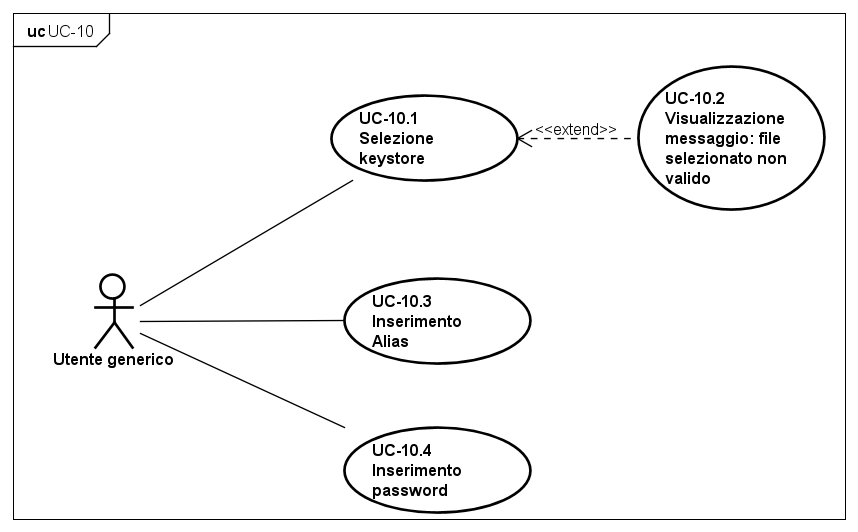
\includegraphics[width=10cm, height=8cm]{./immagini/usecase/uc_10.png}
    \caption{Sotto-casi d'uso UC-10 Firmare l'APK ricompilato}
\end{figure}

\subsection{UC-11 Visualizzazione credenziali keystore errati}\label{subsec:uc-11-visualizzazione-credenziali-keystore-errati}
\begin{itemize}
    \item \textbf{attori:} utente generico;
    \item \textbf{scopo:}  mostrare all'utente il messaggio di errore delle credenziali relativa al keystore;
    \item \textbf{descrizione:} per firmare l'APK l'utente è deve inserire dei credenziali, e quando quest'ultimi sono errati viene mostrato un messaggio di errore;
    \item \textbf{pre-condizioni:} l'utente ha selezionato la funzionalità per ricompilare l'APK;
    \item \textbf{post-condizioni:} l'utente ha visualizzato il messaggio di errore;
    \item \textbf{flusso degli eventi principali:}
    \begin{itemize}
        \item l'utente ha visualizzato l'errore;
    \end{itemize}
\end{itemize}

\subsection{UC-12 Visualizzazione messaggio file non valido}\label{subsec:uc-12-visualizzazione-messaggio-file-non-valido}
\begin{itemize}
    \item \textbf{attori:} utente generico;
    \item \textbf{scopo:} mostrare il messaggio di errore se seleziona un file non valido;
    \item \textbf{descrizione:} quando l'utente seleziona un file che non ha l'estensione APK un messaggio deve essere mostrato all'utente;
    \item \textbf{pre-condizioni:} l'utente ha selezionato un file non APK;
    \item \textbf{post-condizioni:} l'utente ha visualizzato il messaggio d'errore;
    \item \textbf{flusso degli eventi principali:}
    \begin{itemize}
        \item l'utente visualizza il messaggio d'errore.
    \end{itemize}
\end{itemize}
\subsection{UC-13 Decodifica dei file \textit{.dex} in file \textit{.java}}\label{subsec:uc-13-decodifica-dei-filetextitin-filetextit}
\begin{itemize}
    \item \textbf{attori:} utente generico;
    \item \textbf{scopo:} decodifica dei file .dex in class quindi da class in java;
    \item \textbf{descrizione:} dall'APK ricompilato si ottengono dei file \textit{.dex} che possono essere convertiti in \textit{.class} e quindi in \textit{.java};
    \item \textbf{pre-condizioni:} la decompilazione dell'APK \`{e} andata a buon fine;
    \item \textbf{post-condizioni:} la decodifica dei file \textit{.dex} in \textit{.java} \`{e} andata a buon fine;
    \item \textbf{flusso degli eventi principali:}
    \begin{itemize}
        \item l'utente seleziona la voce "Decodifica Dex".
    \end{itemize}
\end{itemize}
\begin{figure}[H]
    \centering
    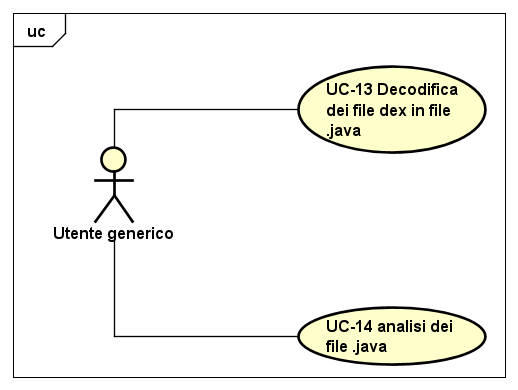
\includegraphics[width=10cm, height=8cm]{./immagini/usecase/UC-13_14.png}
    \caption{Casi d'uso 13 e 14}
\end{figure}
\subsection{UC-14 Analisi del codice \textit{.java}}\label{subsec:uc-14-analisi-del-codicetextit}
\begin{itemize}
    \item \textbf{attori:} attore generico;
    \item \textbf{scopo:} permettere di effettuare dell'analisi sul codice;
    \item \textbf{descrizione:} dopo aver ottenuto i file \textit{.java} eseguendo il caso d'uso UC-13, si potr\`{a} effettuare dell'analisi sul codice;
    \item \textbf{pre-condizioni:} la decodifica dei file \textit{.dex} in \textit{.java} \`{e} andata a buon fine;
    \item \textbf{post-condizioni:} viene generato un pdf con i risultati dell'analisi;
    \item \textbf{flusso degli eventi principali:}
    \begin{itemize}
        \item l'utente seleziona la voce "analyze";
        \item l'utente seleziona le opzioni di analisi;
        \item all'analisi completato, l'utente specifica dove posizionare il file pdf con i risultati dell'analisi;
        \item il file viene salvato nel percorso da lui specificato.
    \end{itemize}
\end{itemize}
\begin{figure}[H]
    \centering
    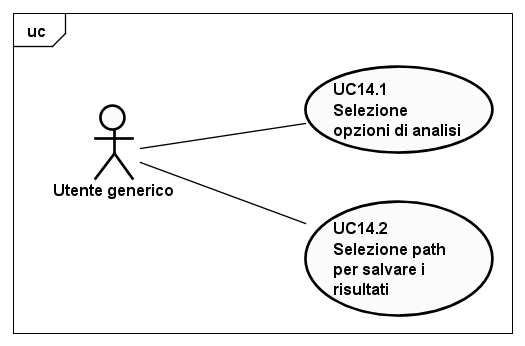
\includegraphics[width=10cm, height=8cm]{./immagini/usecase/uc_14_1_14_2.png}
    \caption{Sottocasi d'uso del caso d'uso 14}
\end{figure}
